\section{System-wide Profiling \& Tracing}

\begin{frame}
  \frametitle{System-wide Profiling \& Tracing}
  \begin{itemize}
    \item Sometimes, the problems are not tied to an application but rather
          due to the usage of multiple layers (drivers, application, kernel).
    \item In that case, it might be useful to analyze the whole stack.
    \item The kernel already includes a large number of tracepoints that can be
          recorded using specific tools.
    \item New tracepoints can also be created statically or dynamically using
          various mechanisms (kprobes for instance).
  \end{itemize}
\end{frame}

\begin{frame}[fragile]
  \frametitle{Kprobes}
  \begin{itemize}
    \item {Kprobes} allows to insert breaks at almost any kernel address
          dynamically and allows to extract debugging and performance
          information
    \item Uses code patching to modify text code to insert calls to specific
          handlers
    \begin{itemize}
      \item \code{kprobes} allows to execute specific handlers when the hooked
            instruction is executed
      \item \code{kretprobes} will trigger when returning from a function allowing to
            extract the return value of functions but also display the
            parameters that were used for the function call
    \end{itemize}
    \item Support should be enabled using \kconfigval{CONFIG_KPROBES}{y}
    \item Moreover, since probes are inserted using modules, \kconfigval{CONFIG_MODULES}{y}
    and \kconfigval{CONFIG_MODULE_UNLOAD}{y} must be set to be able to
    register probes.
    \item Also requires \kconfigval{CONFIG_KALLSYMS_ALL}{y} when hooking probes
          using \code{symbol_name} field
    \item See \kdochtml{trace/kprobes} for more information
  \end{itemize}
\end{frame}

\begin{frame}[fragile]
  \frametitle{Registering a Kprobe}
  \begin{itemize}
    \item \code{kprobes} can be registered dynamically by loading a module that
          registers a \kstruct{kprobe} with \kfunc{register_kprobe}
    \item Probes should be unregistered at module exit using
          \kfunc{unregister_kprobe}
  \end{itemize}

  \begin{block}{}
    \begin{minted}[fontsize=\small]{C}
struct kprobe probe = {
  .symbol_name = "do_exit",
  .pre_handler = probe_pre;
  .post_handler = probe_post;
};

register_kprobe(&probe);
    \end{minted}
  \end{block}
\end{frame}

\begin{frame}[fragile]
  \frametitle{Registering a kretprobe}
  \begin{itemize}
    \item \code{kretprobes} can be registered the same way than regular probes but using
          a \kstruct{kretprobe} with \kfunc{register_kretprobe}
    \begin{itemize}
      \item Provided handlers will be called on function entry and exit
      \item Probe should be unregistered at module exit using
            \kfunc{unregister_kretprobe}
    \end{itemize}
  \end{itemize}

  \begin{block}{}
    \begin{minted}[fontsize=\small]{C}
int (*kretprobe_handler_t) (struct kretprobe_instance *, struct pt_regs *);
    \end{minted}
  \end{block}

  \begin{block}{}
    \begin{minted}[fontsize=\small]{C}
struct kretprobe probe = {
  .kp.symbol_name = "do_fork",
  .entry_handler = probe_entry;
  .handler = probe_exit;
};

register_kretprobe(&probe);
    \end{minted}
  \end{block}
\end{frame}

\begin{frame}
  \frametitle{{\em perf}}
  \begin{itemize}
    \item {\em perf} allows to do a wide range of tracing and recording operations.
    \item The kernel already contains events and tracepoints that can be used.
          The list is given using \code{perf list}.
    \item Syscall tracepoints should be enabled in kernel configuration using
          \kconfig{CONFIG_FTRACE_SYSCALLS}.
    \item New tracepoint can be created dynamically on all symbols and registers
          when debug info are not present.
    \item Tracing functions, recording variables and parameters content using
          their names will require a kernel compiled with
          \kconfig{CONFIG_DEBUG_INFO}.
    \item If perf does not find \code{vmlinux} you have to provide it
          using \code{-k <vmlinux>}.
  \end{itemize}
\end{frame}

\begin{frame}[fragile]
  \frametitle{{\em perf} example}
  \begin{itemize}
    \item List all events that matches \code{syscalls:*}
  \end{itemize}
  \begin{block}{}
    \begin{minted}[fontsize=\footnotesize]{C}
$ perf list syscalls:*
List of pre-defined events (to be used in -e):

  syscalls:sys_enter_accept                          [Tracepoint event]
  syscalls:sys_enter_accept4                         [Tracepoint event]
  syscalls:sys_enter_access                          [Tracepoint event]
  syscalls:sys_enter_adjtimex_time32                 [Tracepoint event]
  syscalls:sys_enter_bind                            [Tracepoint event]
...
    \end{minted}
  \end{block}
  \begin{itemize}
    \item Record all \code{syscalls:sys_enter_read} events for \code{sha256sum}
          command into \code{perf.data} file.
  \end{itemize}
  \begin{block}{}
    \begin{minted}[fontsize=\footnotesize]{C}
$ perf record -e syscalls:sys_enter_read sha256sum /bin/busybox
[ perf record: Woken up 1 times to write data ]
[ perf record: Captured and wrote 0.018 MB perf.data (215 samples) ]
    \end{minted}
  \end{block}
\end{frame}

\begin{frame}[fragile]
  \frametitle{{\em perf report} example}
  \begin{itemize}
    \item Display the collected samples ordered by time spent.
  \end{itemize}
  \begin{block}{}
    \begin{minted}[fontsize=\tiny]{C}
$ perf report
Samples: 591  of event 'cycles', Event count (approx.): 393877062
Overhead  Command      Shared Object                   Symbol
  22,88%  firefox-esr  [nvidia]                        [k] _nv031568rm
   3,21%  firefox-esr  ld-linux-x86-64.so.2            [.] __minimal_realloc
   2,00%  firefox-esr  libc.so.6                       [.] __stpncpy_ssse3
   1,86%  firefox-esr  libglib-2.0.so.0.7400.0         [.] g_hash_table_lookup
   1,62%  firefox-esr  ld-linux-x86-64.so.2            [.] _dl_strtoul
   1,56%  firefox-esr  [kernel.kallsyms]               [k] clear_page_rep
   1,52%  firefox-esr  libc.so.6                       [.] __strncpy_sse2_unaligned
   1,37%  firefox-esr  ld-linux-x86-64.so.2            [.] strncmp
   1,30%  firefox-esr  firefox-esr                     [.] malloc
   1,27%  firefox-esr  libc.so.6                       [.] __GI___strcasecmp_l_ssse3
   1,23%  firefox-esr  [nvidia]                        [k] _nv013165rm
   1,09%  firefox-esr  [nvidia]                        [k] _nv007298rm
   1,03%  firefox-esr  [kernel.kallsyms]               [k] unmap_page_range
   0,91%  firefox-esr  ld-linux-x86-64.so.2            [.] __minimal_free
    \end{minted}
  \end{block}
\end{frame}

\begin{frame}
  \frametitle{{\em perf probe}}
  \begin{itemize}
    \item {\em perf} allows to create dynamic tracepoints on both kernel functions and
          user-space functions.
    \item In order to be able to insert probes, \kconfig{CONFIG_KPROBE} must be
          enabled in the kernel.
    \begin{itemize}
      \item Note: {\em libelf} is required to compile {\em perf} with
            {\em probe} command support.
    \end{itemize}
    \item New dynamic probes can be created and then used using
          {\em perf record}.
    \item Often on embedded platforms, \code{vmlinux} is not present on the
          target and thus only symbols and registers can be used.
  \end{itemize}
\end{frame}

\begin{frame}[fragile]
  \frametitle{{\em perf probe} examples (1/3)}
  \begin{itemize}
    \item List all the kernel symbols that can be probed (no debug info needed):
  \end{itemize}
  \begin{block}{}
    \begin{minted}[fontsize=\scriptsize]{C}
$ perf probe --funcs
    \end{minted}
  \end{block}
  \begin{itemize}
    \item Create a new probe on \code{do_sys_openat2} with {\em filename}
          named parameter (debug info required).
  \end{itemize}
  \begin{block}{}
    \begin{minted}[fontsize=\scriptsize]{C}
$ perf probe --vmlinux=vmlinux_file do_sys_openat2 filename:string
Added new event:
  probe:do_sys_openat2 (on do_sys_openat2 with filename:string)
    \end{minted}
  \end{block}
  \begin{itemize}
    \item Execute \code{tail} and capture previously created probe event:
  \end{itemize}
  \begin{block}{}
    \begin{minted}[fontsize=\scriptsize]{C}
$ perf record -e probe:do_sys_openat2 tail /var/log/messages
...
[ perf record: Woken up 1 times to write data ]
[ perf record: Captured and wrote 0.003 MB perf.data (19 samples) ]
    \end{minted}
  \end{block}
\end{frame}

\begin{frame}[fragile]
  \frametitle{{\em perf probe} examples (2/3)}

  \begin{itemize}
    \item Display the recorded tracepoints with {\em perf script}:
  \end{itemize}
  \begin{block}{}
    \begin{minted}[fontsize=\tiny]{C}
$ perf script
tail   164 [000]  3552.956573: probe:do_sys_openat2: (c02c3750) filename_string="/etc/ld.so.cache"
tail   164 [000]  3552.956642: probe:do_sys_openat2: (c02c3750) filename_string="/lib/tls/v7l/neon/vfp/libresolv.so.2"
...
    \end{minted}
  \end{block}
  \begin{itemize}
    \item Create a new probe on \code{ksys_read} return value using register
          \code{r0} (ARM) alias with "ret" name:
  \end{itemize}
  \begin{block}{}
    \begin{minted}[fontsize=\scriptsize]{C}
$ perf probe ksys_read%return ret=%r0
    \end{minted}
  \end{block}
  \begin{itemize}
    \item Execute \code{sha256sum} and capture previously created probe events:
  \end{itemize}
  \begin{block}{}
    \begin{minted}[fontsize=\scriptsize]{C}
$ perf record -e probe:ksys_read__return sha256sum /etc/fstab
    \end{minted}
  \end{block}
\end{frame}

\begin{frame}[fragile]
  \frametitle{{\em perf probe} examples (3/3)}

  \begin{itemize}
    \item List all probes that have been created:
  \end{itemize}
  \begin{block}{}
    \begin{minted}[fontsize=\scriptsize]{C}
$ perf probe -l
  probe:ksys_read__return (on ksys_read%return with ret)
    \end{minted}
  \end{block}
  \begin{itemize}
    \item Remove an existing tracepoint:
  \end{itemize}
  \begin{block}{}
    \begin{minted}[fontsize=\tiny]{C}
$ perf probe -d probe:ksys_read__return
    \end{minted}
  \end{block}
\end{frame}

\begin{frame}[fragile]
  \frametitle{{\em perf record} example}

  \begin{itemize}
    \item Record all events for all cpus (system-wide mode):
  \end{itemize}
  \begin{block}{}
    \begin{minted}[fontsize=\scriptsize]{console}
$ perf record -a
^C
    \end{minted}
  \end{block}
  \begin{itemize}
    \item Display recorded events from perf.data using \code{perf script}
  \end{itemize}
  \begin{block}{}
    \begin{minted}[fontsize=\tiny]{console}
$ perf script
...
klogd    85 [000]   208.609712:     116584   cycles:          b6dd551c memset+0x2c (/lib/libc.so.6)
klogd    85 [000]   208.609898:     121267   cycles:          c0a44c84 _raw_spin_unlock_irq+0x34 (vmlinux)
klogd    85 [000]   208.610094:     127434   cycles:          c02f3ef4 kmem_cache_alloc+0xd0 (vmlinux)
 perf   130 [000]   208.610311:     132915   cycles:          c0a44c84 _raw_spin_unlock_irq+0x34 (vmlinux)
 perf   130 [000]   208.619831:     143834   cycles:          c0a44cf4 _raw_spin_unlock_irqrestore+0x3c (vmlinux)
klogd    85 [000]   208.620048:     143834   cycles:          c01a07f8 syslog_print+0x170 (vmlinux)
klogd    85 [000]   208.620241:     126328   cycles:          c0100184 vector_swi+0x44 (vmlinux)
klogd    85 [000]   208.620434:     128451   cycles:          c096f228 unix_dgram_sendmsg+0x46c (vmlinux)
kworker/0:2-mm_    44 [000]   208.620653:     133104   cycles:          c0a44c84 _raw_spin_unlock_irq+0x34 (vmlinux)
 perf   130 [000]   208.620859:     138065   cycles:          c0198460 lock_acquire+0x184 (vmlinux)
...
    \end{minted}
  \end{block}
\end{frame}

\begin{frame}[fragile]
  \frametitle{Using {\em perf trace} }
  \begin{itemize}
    \item \code{perf trace} captures and display all tracepoints/events that
          have been triggered when executing a command
  \end{itemize}

  \begin{block}{}
    \begin{minted}[fontsize=\tiny]{console}
$ perf trace -e "net:*" ping -c 1 192.168.1.1
PING 192.168.1.1 (192.168.1.1) 56(84) bytes of data.
      0.000 ping/37820 net:net_dev_queue(skbaddr: 0xffff97bbc6a17900, len: 98,
        name: "enp34s0")
      0.005 ping/37820 net:net_dev_start_xmit(name: "enp34s0",
        skbaddr: 0xffff97bbc6a17900, protocol: 2048, len: 98,
        network_offset: 14, transport_offset_valid: 1, transport_offset: 34)
      0.009 ping/37820 net:net_dev_xmit(skbaddr: 0xffff97bbc6a17900, len: 98,
        name: "enp34s0")
64 bytes from 192.168.1.1: icmp_seq=1 ttl=64 time=0.867 ms
    \end{minted}
  \end{block}
\end{frame}

\begin{frame}[fragile]
  \frametitle{Using {\em perf top} }
  \begin{itemize}
    \item \code{perf top} allows to do a live analysis of the running kernel
    \item It will sample all function calls and display them ordered by most
          time consuming one.
    \item This allows to profile the whole system usage
  \end{itemize}

  \begin{block}{}
    \begin{minted}[fontsize=\tiny]{console}
$ perf top
Samples: 19K of event 'cycles', 4000 Hz, Event count (approx.): 4571734204 lost: 0/0 drop: 0/0
Overhead  Shared Object                         Symbol
   2,01%  [nvidia]                              [k] _nv023368rm
   0,94%  [kernel]                              [k] __static_call_text_end
   0,89%  [vdso]                                [.] 0x0000000000000655
   0,81%  [nvidia]                              [k] _nv027733rm
   0,79%  [kernel]                              [k] clear_page_rep
   0,76%  [kernel]                              [k] psi_group_change
   0,70%  [kernel]                              [k] check_preemption_disabled
   0,69%  code                                  [.] 0x000000000623108f
   0,60%  code                                  [.] 0x0000000006231083
   0,59%  [kernel]                              [k] preempt_count_add
   0,54%  [kernel]                              [k] module_get_kallsym
   0,53%  [kernel]                              [k] copy_user_generic_string
    \end{minted}
  \end{block}
\end{frame}

\begin{frame}
  \frametitle{ftrace}
  \begin{itemize}
    \item {\em ftrace} is a tracing framework within the kernel which stands for
          "Function Tracer".
    \item It offers a wide range of tracing capabilities allowing to observe the
          system behavior.
    \begin{itemize}
      \item Trace static tracepoints already inserted in the kernel various
            parts (scheduler, interrupts, etc).
      \item Relies on GCC mcount() capability and kernel code patching mechanism
            to call {\em ftrace} tracing handlers.
    \end{itemize}
    \item All traces are recorded in a ring buffer that is optimized for tracing.
    \item Uses {\em tracefs} filesystem to control and display tracing events.
    \begin{itemize}
      \item \codewithhash{\# mount -t tracefs nodev /sys/kernel/tracing}.
    \end{itemize}
    \item {\em ftrace} support must be enabled in the kernel using
          \kconfigval{CONFIG_FTRACE}{y}.
    \item \kconfig{CONFIG_DYNAMIC_FTRACE} allows to have a zero overhead tracing
          support.
  \end{itemize}
\end{frame}

\begin{frame}
  \frametitle{ftrace files}
  \begin{itemize}
    \item {\em ftrace} controls are exposed through some specific files located under
          \code{/sys/kernel/tracing}.
    \begin{itemize}
      \item \code{current_tracer}: Current tracer that is used.
      \item \code{available_tracers}: List of available tracers that are
            compiled in the kernel.
      \item \code{tracing_on}: Enable/disable tracing.
      \item \code{trace}: Acquired trace in human readable format. Format will
            differ depending on the tracer used.
      \item \code{trace_marker{_raw}}: Emit comments from userspace in the
            trace buffer.
      \item \code{set_ftrace_filter}: Filter some specific functions.
      \item \code{set_graph_function}: Graph only the specified functions child.
    \end{itemize}
    \item Many other files are exposed, see \kdochtml{trace/ftrace}.
    \item {\em trace-cmd} CLI and {\em Kernelshark} GUI tools allow to record
          and visualize tracing data more easily.
  \end{itemize}
\end{frame}

\begin{frame}[fragile]
  \frametitle{ftrace tracers}
  \begin{itemize}
    \item ftrace provides several "tracers" which allow to trace different things.
    \item The tracer to be used should be written to the \code{current_tracer} file
    \begin{itemize}
      \item \code{nop}: Trace nothing, used to disable all tracing.
      \item \code{function}: Trace all kernel functions that are called.
      \item \code{function_graph}: Similar to \code{function} but traces both entry and exit.
      \item \code{hwlat}: Trace hardware latency.
      \item \code{irqsoff}: Trace sections where interrupts are disabled.
      \item \code{branch}: Trace likely()/unlikely() prediction errors.
      \item \code{mmiotrace}: Trace all accesses to the hardware (\code{read[bwlq]/write[bwlq]}).
    \end{itemize}
    \item \textbf{Warning: Some tracers can be expensive!}
  \end{itemize}
  \begin{block}{}
    \begin{minted}[fontsize=\small]{console}
# echo "function" > /sys/kernel/tracing/current_tracer
    \end{minted}
  \end{block}
\end{frame}

\begin{frame}[fragile]
  \frametitle{{\em function\_graph} tracer report example}
  \begin{itemize}
    \item The {\em function\_graph} traces all the function that
      executed and their associated callgraphs
    \item Will display the process, CPU, timestamp and function graph:
  \end{itemize}
  \begin{block}{}
    \begin{minted}[fontsize=\tiny]{console}
$ trace-cmd report
...
dd-113   [000]   304.526590: funcgraph_entry:                   |  sys_write() {
dd-113   [000]   304.526597: funcgraph_entry:                   |    ksys_write() {
dd-113   [000]   304.526603: funcgraph_entry:                   |      __fdget_pos() {
dd-113   [000]   304.526609: funcgraph_entry:        6.541 us   |        __fget_light();
dd-113   [000]   304.526621: funcgraph_exit:       + 18.500 us  |      }
dd-113   [000]   304.526627: funcgraph_entry:                   |      vfs_write() {
dd-113   [000]   304.526634: funcgraph_entry:        6.334 us   |        rw_verify_area();
dd-113   [000]   304.526646: funcgraph_entry:        6.208 us   |        write_null();
dd-113   [000]   304.526658: funcgraph_entry:        6.292 us   |        __fsnotify_parent();
dd-113   [000]   304.526669: funcgraph_exit:       + 43.042 us  |      }
dd-113   [000]   304.526675: funcgraph_exit:       + 78.833 us  |    }
dd-113   [000]   304.526680: funcgraph_exit:       + 91.291 us  |  }
dd-113   [000]   304.526689: funcgraph_entry:                   |  sys_read() {
dd-113   [000]   304.526695: funcgraph_entry:                   |    ksys_read() {
dd-113   [000]   304.526702: funcgraph_entry:                   |      __fdget_pos() {
dd-113   [000]   304.526708: funcgraph_entry:        6.167 us   |        __fget_light();
dd-113   [000]   304.526719: funcgraph_exit:       + 18.083 us  |      }
    \end{minted}
  \end{block}
\end{frame}

\begin{frame}
  \frametitle{{\em irqsoff} tracer}
  \begin{itemize}
    \item ftrace {\em irqsoff} tracer allows to trace the irqs latency due to
          interrupts being disabled for too long.
    \item Helpful to find why interrupts have high latencies on a system.
    \item This tracer will record the longest trace with interrupts being disabled.
    \item This tracer needs to be enabled with \kconfigval{IRQSOFF_TRACER}{y}.
    \begin{itemize}
      \item \code{preemptoff}, \code{premptirqsoff} tracers also exist to trace
            section of code were preemption is disabled.
    \end{itemize}
  \end{itemize}
  \center\includegraphics[height=0.25\textheight]{slides/debugging-system-wide-profiling/kernel_irqsoff.pdf}
\end{frame}

\begin{frame}[fragile]
  \frametitle{{\em irqsoff} tracer report example}
  \begin{block}{}
    \begin{minted}[fontsize=\tiny]{console}
# latency: 276 us, #104/104, CPU#0 | (M:preempt VP:0, KP:0, SP:0 HP:0 #P:2)
#    -----------------
#    | task: stress-ng-114 (uid:0 nice:0 policy:0 rt_prio:0)
#    -----------------
#  => started at: __irq_usr
#  => ended at:   irq_exit
#
#
#                    _------=> CPU#            
#                   / _-----=> irqs-off        
#                  | / _----=> need-resched    
#                  || / _---=> hardirq/softirq 
#                  ||| / _--=> preempt-depth   
#                  |||| /     delay            
#  cmd     pid     ||||| time  |   caller      
#     \   /        |||||  \    |   /         
stress-n-114       0d...    2us : __irq_usr
stress-n-114       0d...    7us : gic_handle_irq <-__irq_usr
stress-n-114       0d...   10us : __handle_domain_irq <-gic_handle_irq
...
stress-n-114       0d...  270us : __local_bh_disable_ip <-__do_softirq
stress-n-114       0d.s.  275us : __do_softirq <-irq_exit
stress-n-114       0d.s.  279us+: tracer_hardirqs_on <-irq_exit
stress-n-114       0d.s.  290us : <stack trace>
    \end{minted}
  \end{block}
\end{frame}

\begin{frame}
  \frametitle{Hardware latency detector}
  \begin{itemize}
    \item ftrace {\em hwlat} tracer will help to find if the hardware generates
          latency.
    \begin{itemize}
      \item Sytem Management interrupts for instance are non maskable and
            directly trigger some firmware support feature, suspending CPU execution.
      \item Interrupts handled by secure monitor can also cause this kind of
            latency.
    \end{itemize}
    \item If some latency is found with this tracer, the system is probably
          not suitable for real time usage.
    \item Uses a single core looping while interrupts are disabled and measuring
          the time elapsed between two consecutive time reads.
    \item Needs to be builtin the kernel with \kconfigval{CONFIG_HWLAT_TRACER}{y}.
  \end{itemize}

  \center\includegraphics[height=0.25\textheight]{slides/debugging-system-wide-profiling/kernel_hwlat.pdf}
\end{frame}

\begin{frame}[fragile]
  \frametitle{\kfunc{trace_printk}}
  \begin{itemize}
    \item \kfunc{trace_printk} allows to emit strings in the trace buffer
    \item Useful to trace some specific conditions in your code and display it in the trace buffer 
  \end{itemize}
  \begin{block}{}
    \begin{minted}[fontsize=\tiny]{C}
#include <linux/ftrace.h>
void read_hw()
{
  if (condition)
    trace_printk("Condition is true!");
}
    \end{minted}
  \end{block}
  \begin{itemize}
    \item Will display the following in the trace buffer for \code{function_graph} tracer
  \end{itemize}
  \begin{block}{}
    \begin{minted}[fontsize=\tiny]{console}
1)               |             read_hw() {
1)               |                /* Condition is true! */
1)   2.657 us    |             }
    \end{minted}
  \end{block}
\end{frame}

\begin{frame}
  \frametitle{{\em trace-cmd}}
  \begin{itemize}
    \item {\em trace-cmd} is a tool written by Steven Rostedt which allows
          interacting with {\em ftrace} (\manpage{trace-cmd}{1}).
    \item The tracers supported by {\em trace-cmd} are those exposed by ftrace.
    \item {\em trace-cmd} offers multiple commands:
    \begin{itemize}
      \item {\em list}: List available plugins/events that can be recorded.
      \item {\em record}: Record a trace into the file \code{trace.dat}.
      \item {\em report}: Display \code{trace.dat} acquisition results.
    \end{itemize}
    \item At the end of recording, a \code{trace.dat} file will be generated.
  \end{itemize}
\end{frame}

\begin{frame}
  \frametitle{Remote tracing with {\em trace-cmd}}
  \begin{itemize}
    \item {\em trace-cmd} output can be quite big and thus difficult to
          store on an embedded platform with limited storage.
    \item For that purpose, a \code{listen} command is available and allows sending
          the acquisitions over the network:
    \begin{itemize}
      \item Run \code{trace-cmd listen -p 6578} on the remote system that will
            be collecting the traces
      \item On the target system, use \code{trace-cmd record -N <target_ip>:6578}
            to specify the remote system that will collect the traces
    \end{itemize}
  \end{itemize}
  \center\includegraphics[height=0.15\textheight]{slides/debugging-system-wide-profiling/ftrace-remote.pdf}
\end{frame}

\begin{frame}[fragile]
  \frametitle{{\em trace-cmd} examples (1/3)}
  \begin{itemize}
    \item List available tracers
  \end{itemize}
  \begin{block}{}
    \begin{minted}[fontsize=\tiny]{console}
$ trace-cmd list -t
blk mmiotrace function_graph function nop
    \end{minted}
  \end{block}
  \begin{itemize}
    \item List available events
  \end{itemize}
  \begin{block}{}
    \begin{minted}[fontsize=\tiny]{console}
$ trace-cmd list -e
...
migrate:mm_migrate_pages_start
migrate:mm_migrate_pages
tlb:tlb_flush
syscalls:sys_exit_process_vm_writev
...
    \end{minted}
  \end{block}
  
  \begin{itemize}
    \item List available functions for filtering with \code{function} and
        \code{function_graph} tracers
  \end{itemize}
  \begin{block}{}
    \begin{minted}[fontsize=\tiny]{console}
$ trace-cmd list -f
...
wait_for_initramfs
__ftrace_invalid_address___64
calibration_delay_done
calibrate_delay
...
    \end{minted}
  \end{block}


\end{frame}

\begin{frame}[fragile]
  \frametitle{{\em trace-cmd} examples (2/3)}
  \begin{itemize}
    \item Start the function tracer and record data globally on the system
  \end{itemize}
  \begin{block}{}
    \begin{minted}[fontsize=\tiny]{console}
$ trace-cmd record -p function
    \end{minted}
  \end{block}

  \begin{itemize}
    \item Use the function tracer but filter only \code{spi_*} functions
  \end{itemize}
  \begin{block}{}
    \begin{minted}[fontsize=\tiny]{console}
$ trace-cmd record -l spi_* -p function
    \end{minted}
  \end{block}

  \begin{itemize}
    \item Trace the {\em dd} command using the function graph tracer:
  \end{itemize}
  \begin{block}{}
    \begin{minted}[fontsize=\tiny]{console}
$ trace-cmd record -p function_graph dd if=/dev/mmcblk0 of=out bs=512 count=10
    \end{minted}
  \end{block}

  \begin{itemize}
    \item Visualize the data that have been acquired in \code{trace.dat}:
  \end{itemize}
  \begin{block}{}
    \begin{minted}[fontsize=\tiny]{console}
$ trace-cmd report
    \end{minted}
  \end{block}
\end{frame}

\begin{frame}[fragile]
  \frametitle{{\em trace-cmd} examples (3/3)}
  \begin{itemize}
    \item Reset all the {\em ftrace} buffers and remove tracers
  \end{itemize}
  \begin{block}{}
    \begin{minted}[fontsize=\tiny]{console}
$ trace-cmd reset
    \end{minted}
  \end{block}

  \begin{itemize}
    \item Run the {\em irqsoff} tracer on the system:
  \end{itemize}
  \begin{block}{}
    \begin{minted}[fontsize=\tiny]{console}
$ trace-cmd record -p irqsoff
    \end{minted}
  \end{block}
  \begin{itemize}
    \item Record only \code{irq_handler_exit/irq_handler_entry} events on the
          system:
  \end{itemize}
  \begin{block}{}
    \begin{minted}[fontsize=\tiny]{console}
$ trace-cmd record -e irq:irq_handler_exit -e irq:irq_handler_entry
    \end{minted}
  \end{block}

\end{frame}

\begin{frame}[fragile]
  \frametitle{Adding ftrace tracepoints (1/2)}
  \begin{itemize}
    \item For some custom needs, it might be needed to add custom tracepoints
    \item First, one needs to declare the tracepoint definition in a \code{.h}
          file
  \end{itemize}
  \begin{block}{}
    \begin{minted}[fontsize=\footnotesize]{C}
#undef TRACE_SYSTEM
#define TRACE_SYSTEM subsys

#if !defined(_TRACE_SUBSYS_H) || defined(TRACE_HEADER_MULTI_READ)
#define _TRACE_SUBSYS_H

#include <linux/tracepoint.h>

DECLARE_TRACE(subsys_eventname,
        TP_PROTO(int firstarg, struct task_struct *p),
        TP_ARGS(firstarg, p));

#endif /* _TRACE_SUBSYS_H */

/* This part must be outside protection */
#include <trace/define_trace.h>
    \end{minted}
  \end{block}
\end{frame}

\begin{frame}[fragile]
  \frametitle{Adding ftrace tracepoints (2/2)}
  \begin{itemize}
    \item Then, emit tracepoint in a \code{.c} file using that header file
  \end{itemize}
  \begin{block}{}
    \begin{minted}[fontsize=\footnotesize]{C}
#include <trace/events/subsys.h>

#define CREATE_TRACE_POINTS
DEFINE_TRACE(subsys_eventname);

void any_func(void)
{
  ...
  trace_subsys_eventname(arg, task);
  ...
}
    \end{minted}
  \end{block}
  \begin{itemize}
    \item See \kdochtml{trace/tracepoints} for more information
  \end{itemize}
\end{frame}

\begin{frame}[fragile]
  \frametitle{Kernelshark}
  \begin{columns}
    \column{0.65\textwidth}
    \begin{itemize}
      \item Kernelshark is a Qt-based graphical interface for processing
            {\em trace-cmd} trace.dat reports.
      \item Can also setup and acquire data using {\em trace-cmd}.
      \item Displays CPU and tasks as different colors along with the recorded
            events.
      \item Useful when a deep analysis is required for a specific bug.
    \end{itemize}
    \column{0.35\textwidth}
    \vspace{0.5cm}
    \center
\includegraphics[height=0.6\textheight]{slides/debugging-system-wide-profiling/kernelshark-logo.png}
  \end{columns}
\end{frame}

\begin{frame}
  \frametitle{kernelshark}
  \center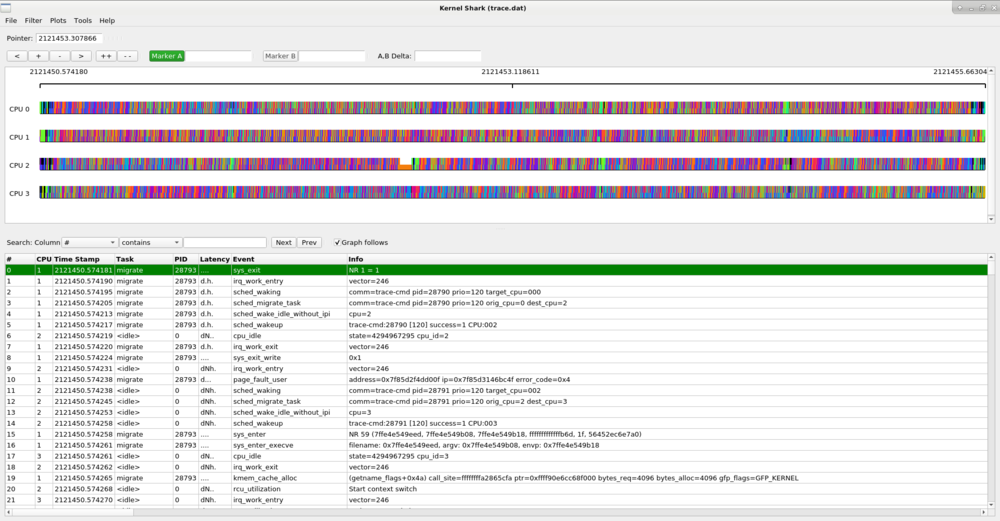
\includegraphics[height=0.8\textheight]{slides/debugging-system-wide-profiling/kernelshark.png}
\end{frame}

\begin{frame}
  \frametitle{eBPF (1/2)}
  \begin{itemize}
    \item BPF stands for Berkeley Packet Filter and was initially used
          for network packet filtering
    \item \href{https://ebpf.io/}{eBPF} framework in the kernel allows running
          user-written BPF programs within the kernel in a safe and efficient
          way (Added in kernel 3.15)
    \item Execution is event-driven and can be hooked using Kprobes, tracepoints
          and other methods of tracing
    \item Executes complex actions and reports data to userspace for
          events that took place in the kernel.
    \item Used to hook into various places of the kernel: VFS, Network stack,
          syscalls, load balancing, security, etc
  \end{itemize}
  \center
\includegraphics[height=0.2\textheight]{slides/debugging-linux-application-stack/logo_ebpf.png}\\ 
  \tiny Image credits: \url{https://ebpf.io/}
\end{frame}

\begin{frame}
  \frametitle{eBPF (2/2)}
  \begin{itemize}
    \item Programs are loaded using the \code{bpf()} system call
          (\manpage{bpf}{2}) and then verified by the kernel BPF verifier before
          being executed.
    \begin{itemize}
      \item Check of privileges to execute BPF program
      \item Verifies that the BPF program always runs to completion and does not
            loop forever
    \end{itemize}
    \item Almost all architectures have a BPF JIT support which allows
          translating the BPF format into native CPU instruction, thus being
          (almost) as fast as natively compiled code
    \item BPF programs can return values in maps of various types (hash tables,
          arrays, etc) which allows sharing data between user-space, eBPF
          programs and kernel space.
    \item Only some functions (called helpers) can be called in eBPF programs.
    \item eBPF programs are attached to events (invoked on trigger).
  \end{itemize}
\end{frame}

\begin{frame}[fragile]
  \frametitle{Writing eBPF programs}
  \begin{itemize}
    \item eBPF programs can be written in (restricted) C and are compiled
          using clang compiler
    \item BCC (BPF Compiler Collection) provides a toolkit to write BPF
          programs more easily using C language (also provides LUA and Python
          front-ends)
    \begin{itemize}
      \item Allows to write tracing and profiling program easily
    \end{itemize}
    \item {\em bpftrace} is a high level language allowing to easily write tracing
          functions
  \end{itemize}
\end{frame}

\begin{frame}[fragile]
  \frametitle{BCC}
  \begin{columns}
    \column{0.75\textwidth}
    \begin{itemize}
      \item BPF Compiler Collection (BCC) is (as its name suggests) a collection
            of BPF based tools.
      \item BCC provides a large number of ready-to-use tools written in BPF.
      \item Also provides an interface to write, load and hook BPF programs more
            easily than using "raw" BPF language.
      \item Available on a large number of architecture (Unfortunately, not arm32).
      \begin{itemize}
        \item On debian, when installed, all tools are named \code{<tool>-bpfcc}.
      \end{itemize}
      \item BCC requires a kernel version >= 4.1.
    \end{itemize}
  \column{0.25\textwidth}
  \vspace{0.5cm}
  
\includegraphics[height=0.2\textheight]{slides/debugging-linux-application-stack/logo_bcc.png}\\ 
  \tiny Image credits: \url{https://github.com/iovisor/bcc}
  \end{columns}
\end{frame}

\begin{frame}[fragile]
  \frametitle{BCC tools}
  \begin{center}
    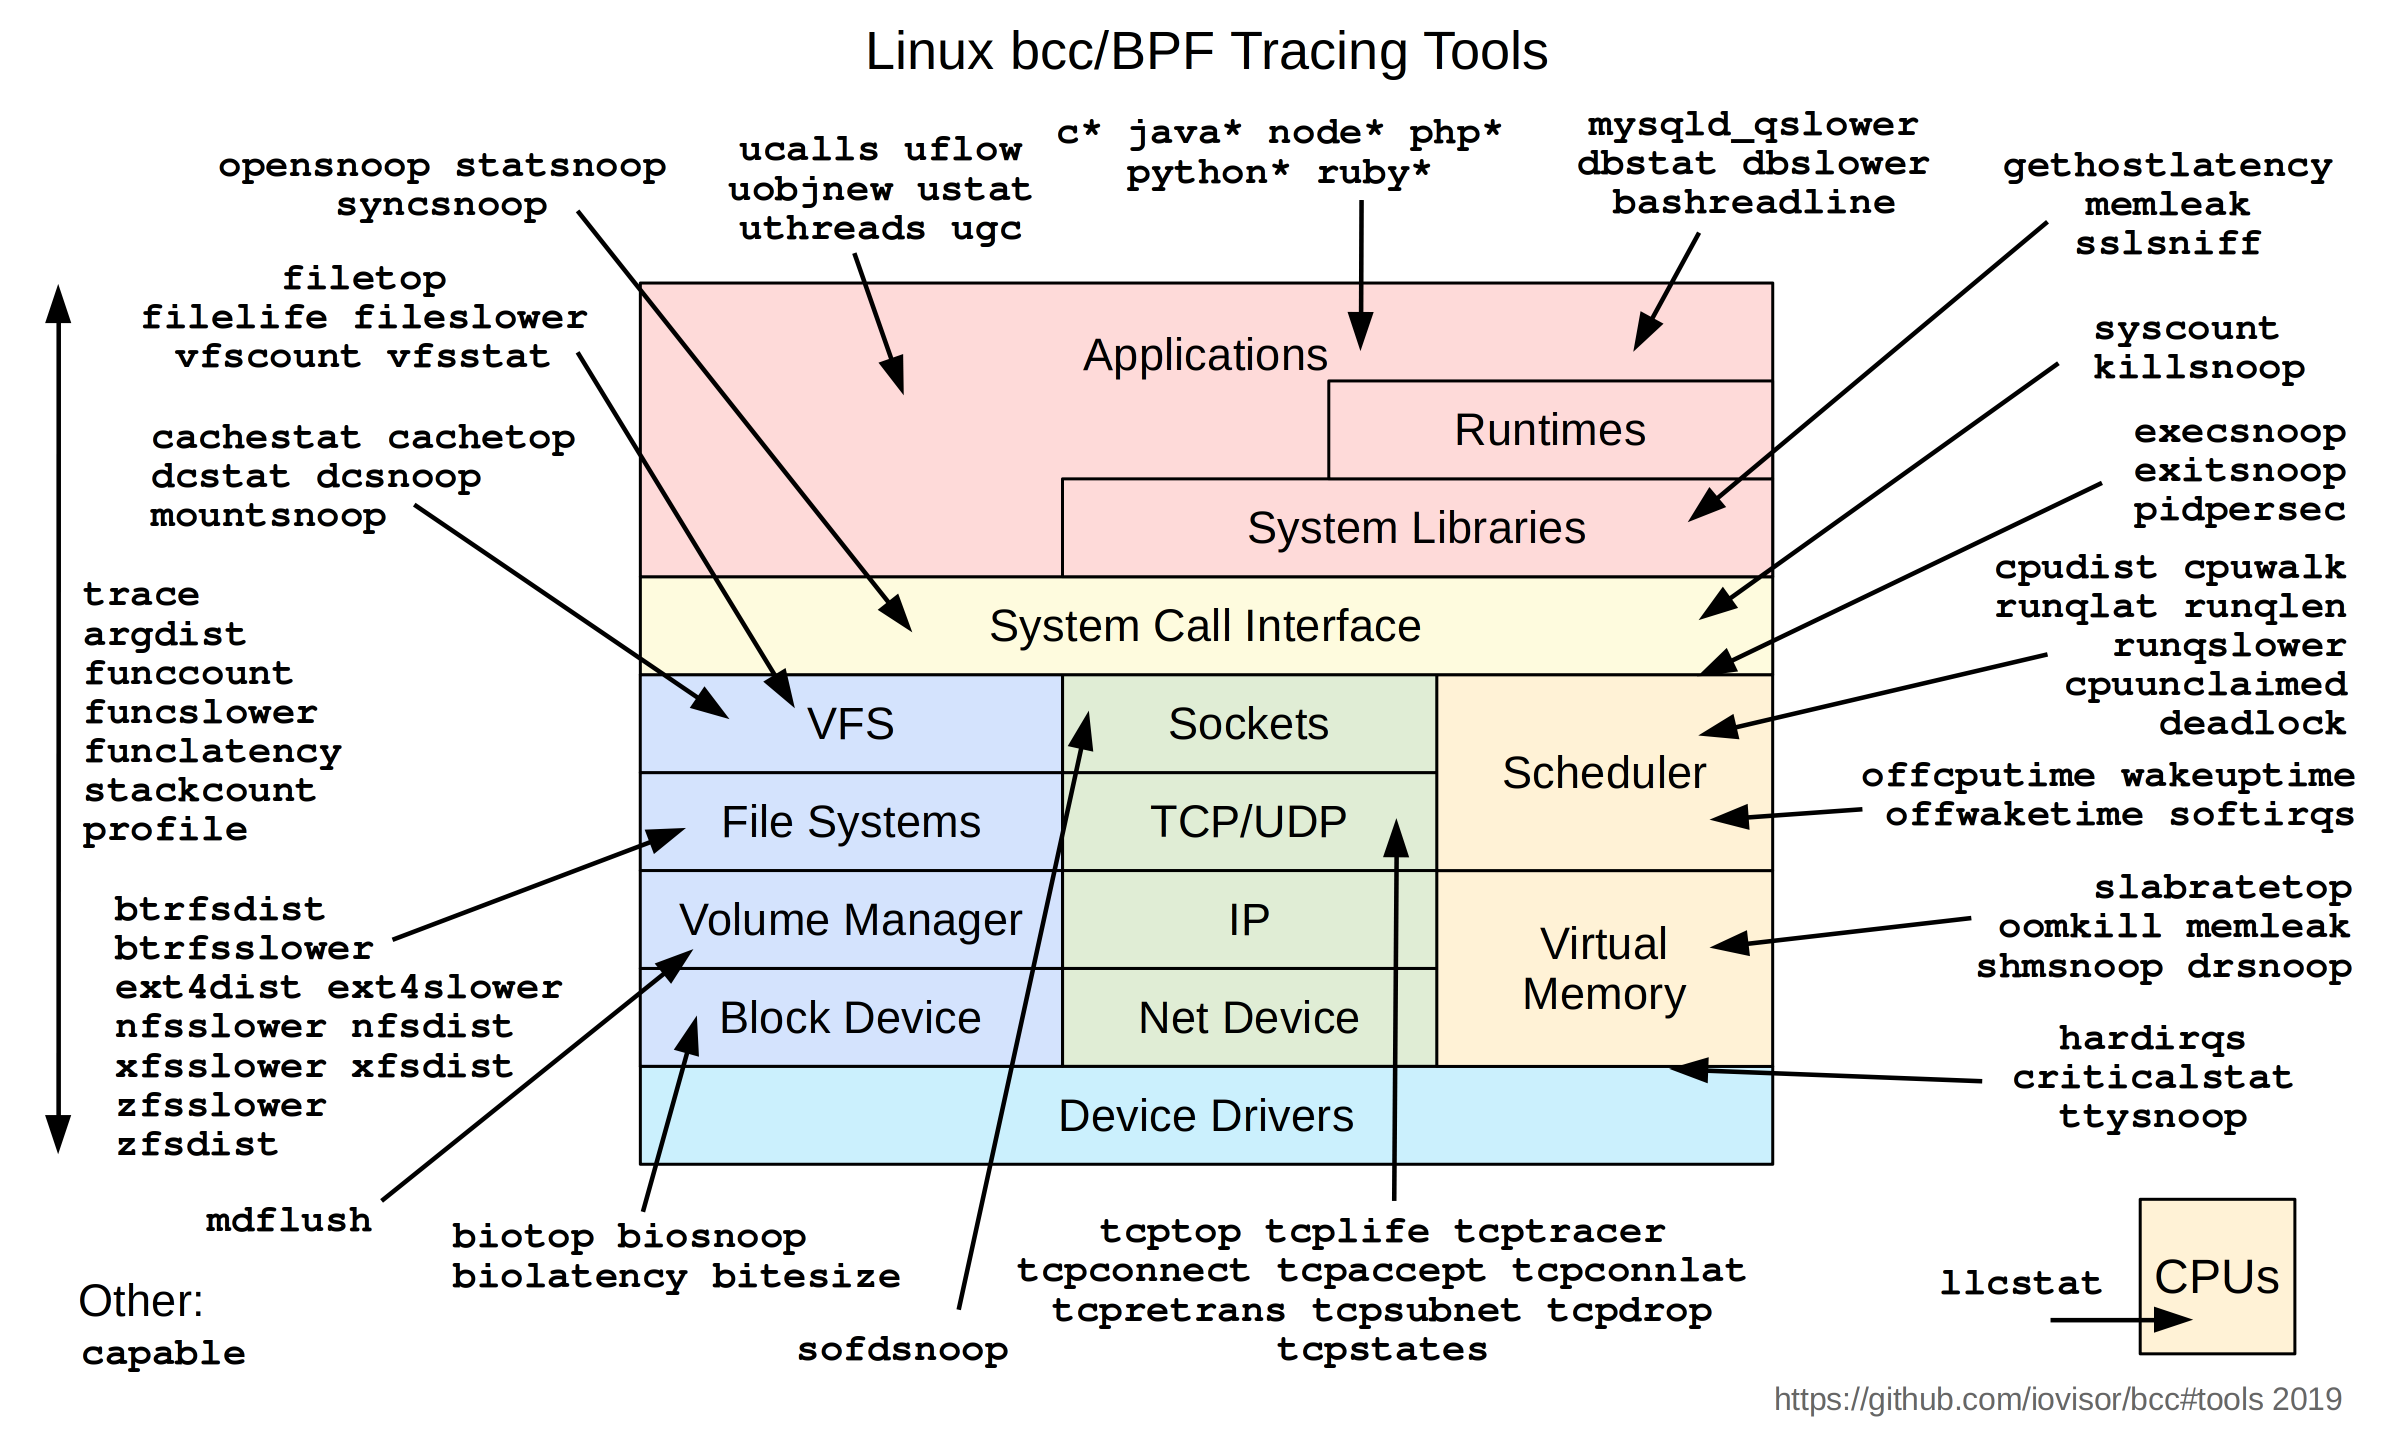
\includegraphics[height=0.8\textheight]{slides/debugging-system-wide-profiling/bcc_tracing_tools_2019.png}\\
    \tiny Image credits: \url{https://www.brendangregg.com/ebpf.html}
  \end{center}
\end{frame}

\begin{frame}[fragile]
  \frametitle{BCC Tools example}
  \begin{itemize}
    \item \code{profile.py} is a CPU profiler allowing to capture stack traces of
          current execution. Its output can be used for flamegraph generation:
  \end{itemize}
  \begin{block}{}
    \begin{minted}[fontsize=\footnotesize]{console}
$ git clone https://github.com/brendangregg/FlameGraph.git
$ profile.py -df -F 99 10 | ./FlameGraph/flamegraph.pl > flamegraph.svg
    \end{minted}
  \end{block}
  \begin{itemize}
    \item \code{tcpconnect.py} script displays all new TCP connection live
  \end{itemize}
  \begin{block}{}
    \begin{minted}[fontsize=\footnotesize]{console}
$ tcpconnect
PID    COMM         IP SADDR            DADDR            DPORT
220321 ssh          6  ::1              ::1              22   
220321 ssh          4  127.0.0.1        127.0.0.1        22   
17676  Chrome_Child 6  2a01:cb15:81e4:8100:37cf:d45b:d87d:d97d 2606:50c0:8003::154 443  
[...]
    \end{minted}
  \end{block}
  \begin{itemize}
    \item And much more to discover at \url{https://github.com/iovisor/bcc}
  \end{itemize}
\end{frame}

\begin{frame}[fragile]
  \frametitle{Using BCC with python}
  \begin{itemize}
    \item BCC python support allows to easily write and hook C program for BPF
          tracing.
    \item Hook with a {\em kprobe} on the \code{clone()} system call and display \verb+"Hello, World!"+ each
          time it is called
  \end{itemize}
  \begin{block}{}
    \begin{minted}[fontsize=\small]{python}
from bcc import BPF

# define BPF program
prog = """
int hello(void *ctx) {
    bpf_trace_printk("Hello, World!\\n");
    return 0;
}
"""
# load BPF program
b = BPF(text=prog)
b.attach_kprobe(event=b.get_syscall_fnname("clone"), fn_name="hello")
    \end{minted}
  \end{block}
\end{frame}

\begin{frame}[fragile]
  \frametitle{bpftrace}
    \begin{columns}
      \column{0.75\textwidth}
      \begin{itemize}
        \item bpftrace is a high level tracing language allowing to write tracing
              expressions easily (\url{https://bpftrace.org/})
        \item Also provide tools to trace various parts of the kernel
        \begin{itemize}
          \item Internally uses LLVM to compile script and BCC to interact with the BPF programs
        \end{itemize}
        \item bpftrace is inspired by awk and C, and predecessor tracers such as DTrace and SystemTap
        \item Rich syntax documented at \url{https://github.com/iovisor/bpftrace/blob/master/docs/reference_guide.md}
      \end{itemize}
    \column{0.25\textwidth}
    \vspace{0.5cm}
    %% Source: https://commons.wikimedia.org/wiki/File:Elf-layout--en.svg
    
\includegraphics[height=0.2\textheight]{slides/debugging-system-wide-profiling/bpftrace.png}\\ 
    \tiny Image credits: \url{https://bpftrace.org/}
  \end{columns}
\end{frame}

\begin{frame}[fragile]
  \frametitle{bpftrace tools}

  \begin{center}
    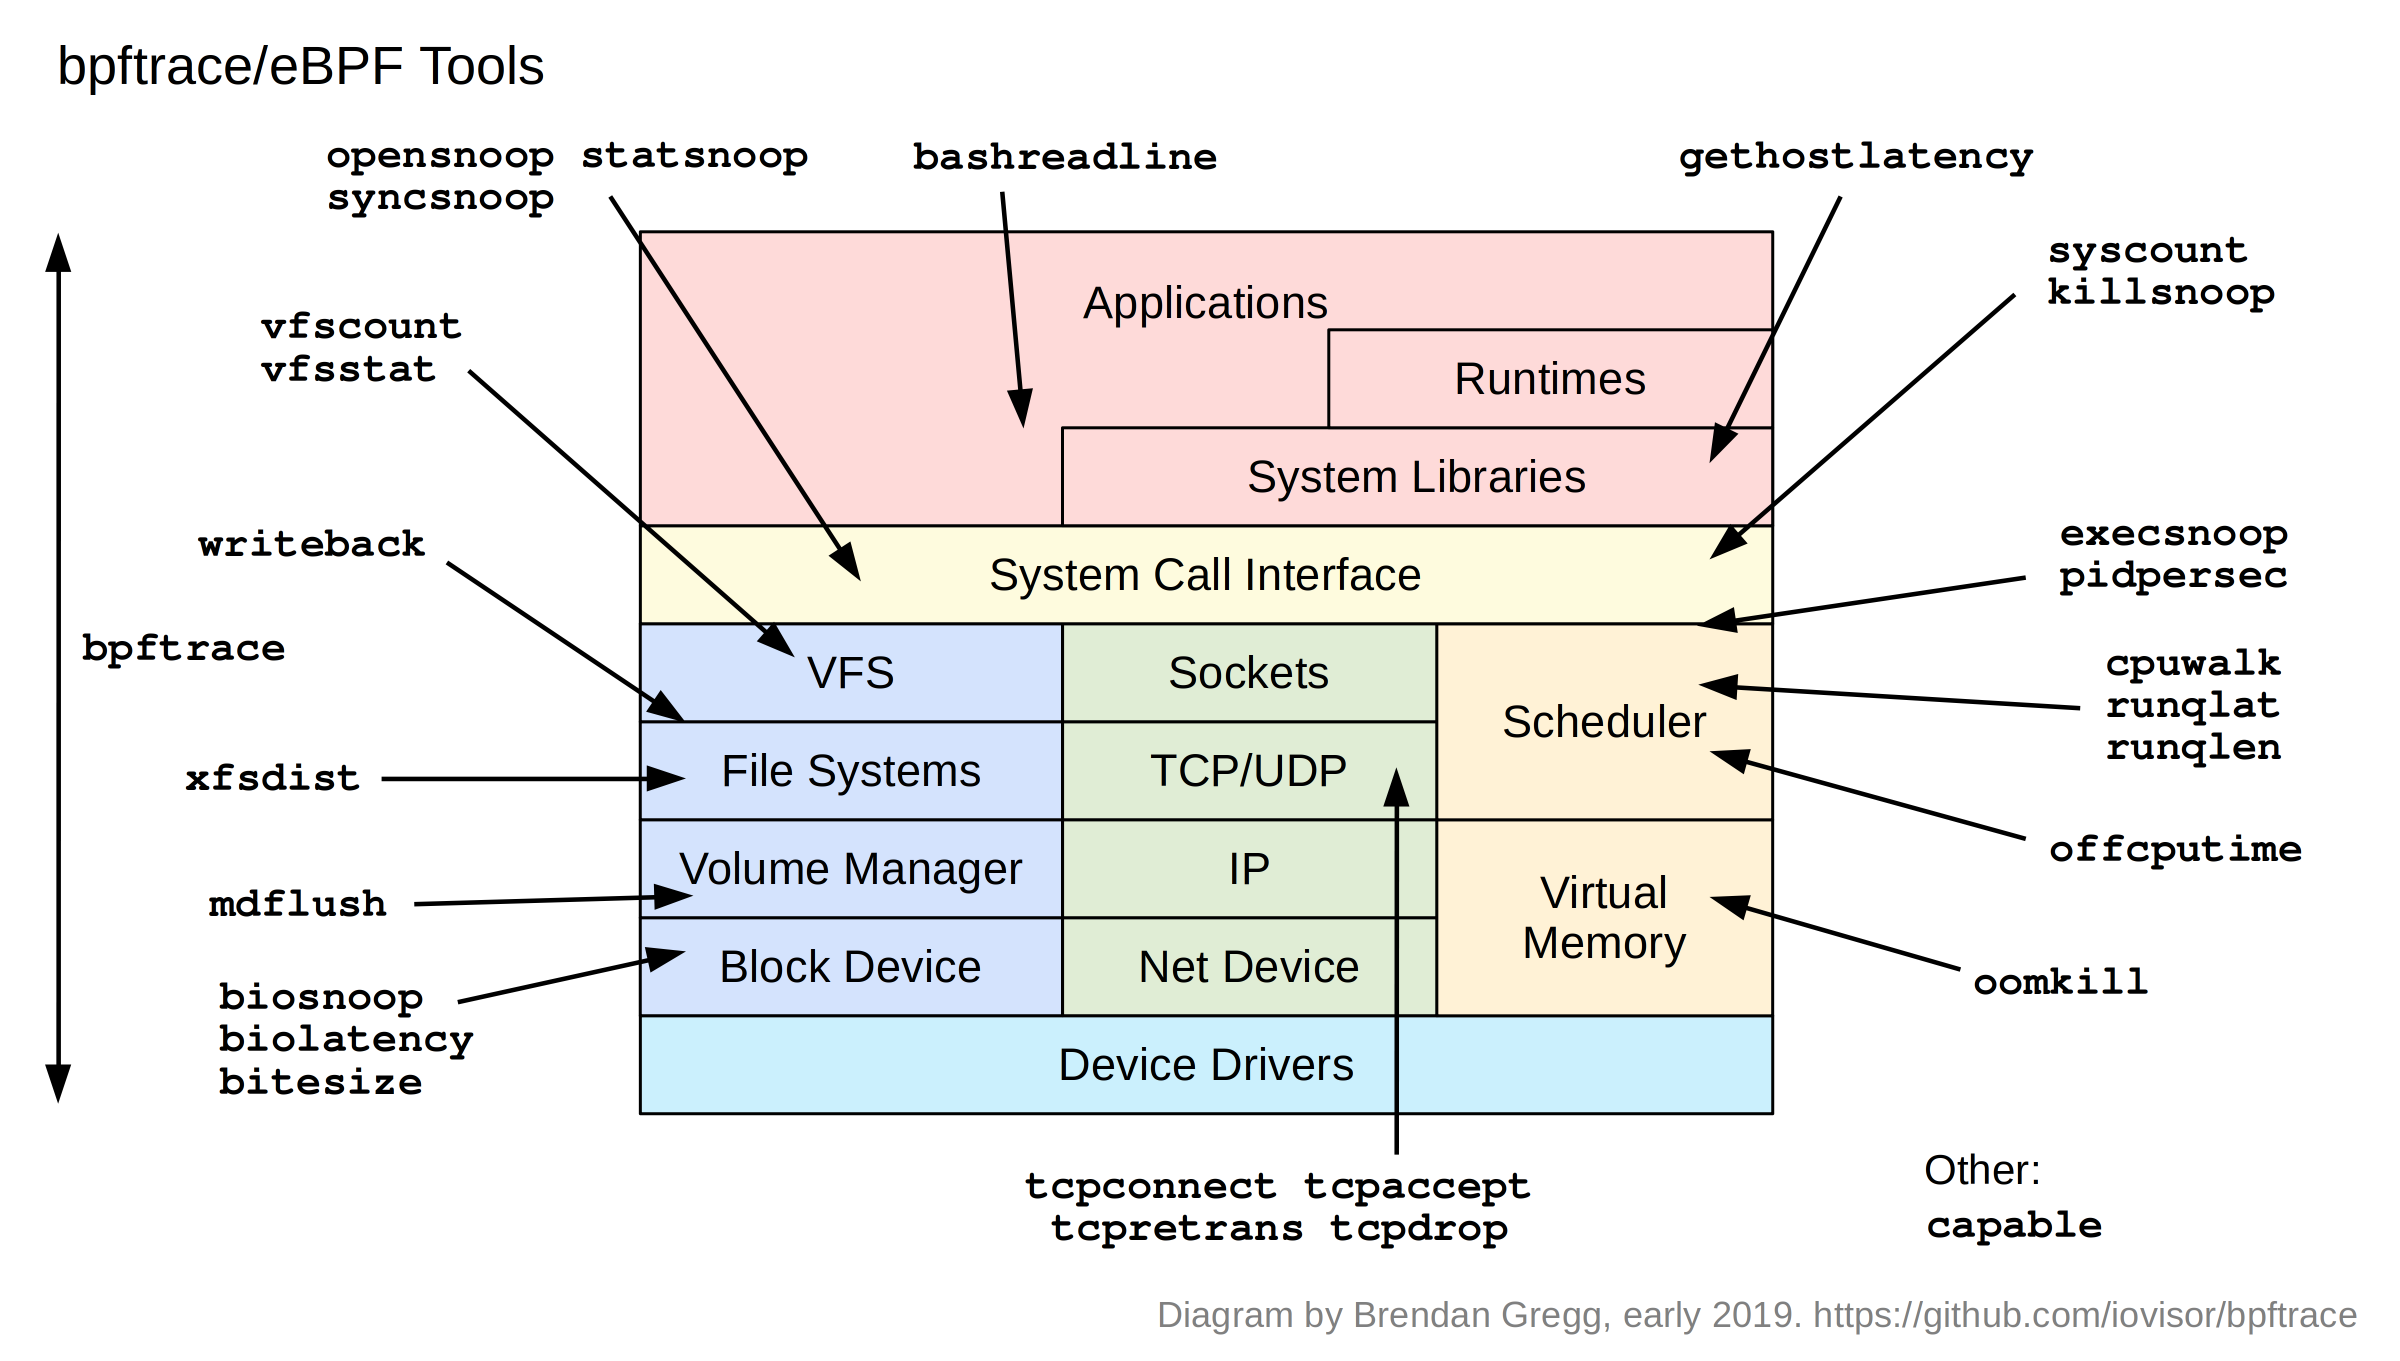
\includegraphics[height=0.8\textheight]{slides/debugging-system-wide-profiling/bpftrace_tools_early2019.png}\\
    \tiny Image credits: \url{https://www.brendangregg.com/ebpf.html}
  \end{center}
\end{frame}

\begin{frame}[fragile]
  \frametitle{Using bpftrace}
  \begin{itemize}
    \item Counting all syscalls per process:
  \end{itemize}
  \begin{block}{}
    \begin{minted}[fontsize=\small]{console}
$ sudo bpftrace -e 'tracepoint:raw_syscalls:sys_enter { @[comm] = count(); }'
Attaching 1 probe...
^C
@[packagekitd]: 1
@[GUsbEventThread]: 1
@[gvfs-afc-volume]: 1
@[ibus-extension-]: 4
    \end{minted}
  \end{block}
\end{frame}

\begin{frame}
  \frametitle{eBPF: resources}
  \begin{itemize}
    \item A Beginner’s Guide to eBPF Programming - Liz Rice, 2020
    \begin{itemize}
      \item Slides: \url{https://speakerdeck.com/lizrice/beginners-guide-to-ebpf}
      \item Video: \url{https://www.youtube.com/watch?v=lrSExTfS-iQ}
      \item Resources: \url{https://github.com/lizrice/ebpf-beginners}
    \end{itemize}
  \end{itemize}
  \begin{center}
     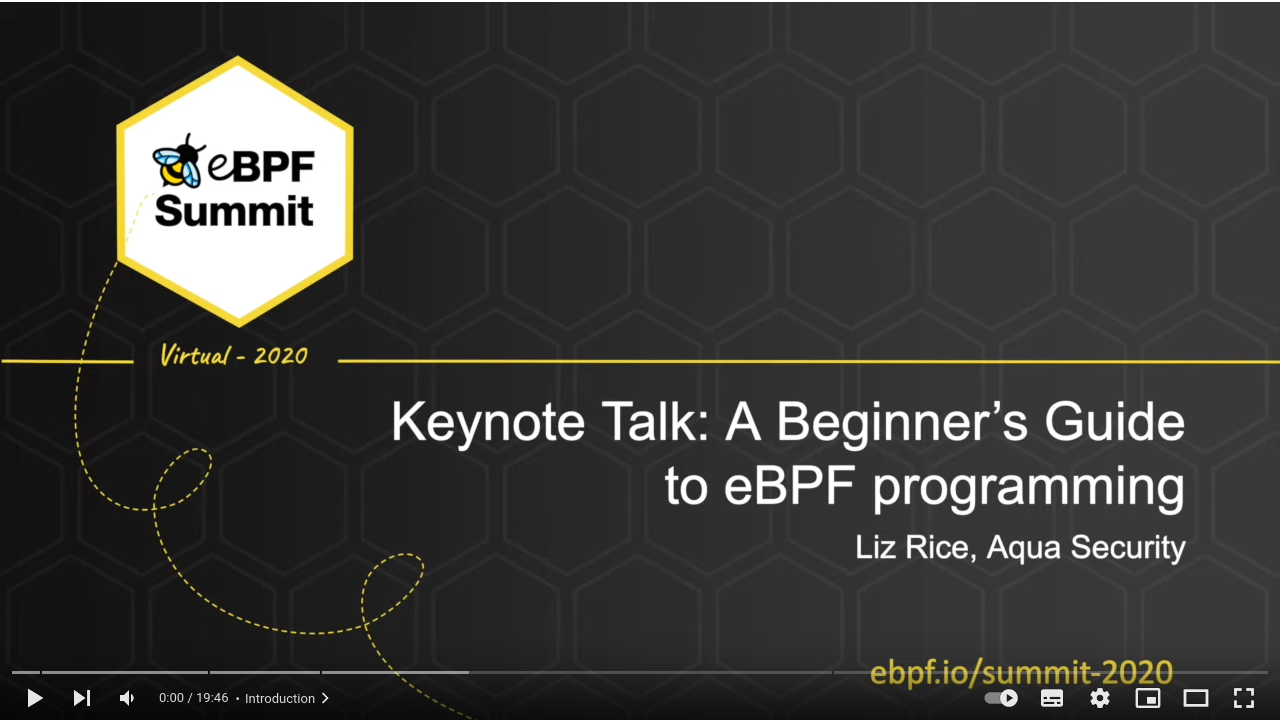
\includegraphics[height=0.6\textheight]{slides/debugging-system-wide-profiling/ebpf_liz_rice_2020.png}
  \end{center}
\end{frame}

\begin{frame}
  \frametitle{{\em LTTng} (1/2)}
  \begin{columns}
    \column{0.65\textwidth}
    \begin{itemize}
      \item LTTng is an open source tracing framework for Linux maintained by
            the \href{https://www.efficios.com/}{EfficiOS} company.
      \item LTTng allows understanding the interactions between the kernel and
            applications (C, C++, Java, Python).
      \begin{itemize}
        \item Also expose a \code{/dev/lttng-logger} that can be used from any
              application.
      \end{itemize}
      \item Tracepoints are associated with a payload (data).
      \item LTTng is focused on low-overhead tracing.
      \item LTTng provides a unified logging of all events (kernel/user).
    \end{itemize}
    \column{0.35\textwidth}
    
\includegraphics[height=0.3\textheight]{slides/debugging-system-wide-profiling/lttng-logo.jpg}
  \end{columns}
\end{frame}

\begin{frame}
  \frametitle{{\em LTTng} (2/2)}
  \begin{itemize}
    \item Uses the \href{https://diamon.org/ctf/}{CTF} trace format (Common
          Trace Format).
    \item LTTng is made of multiple components:
    \begin{itemize}
      \item LTTng-tools: Libraries and command-line interface to control tracing.
      \item LTTng-modules: Linux kernel modules to instrument and trace the kernel.
      \item LTTng-UST: Libraries and Java/Python packages to instrument and trace user applications.
    \end{itemize}
    \item Already packaged by various distribution (debian, fedora, etc) and
          present in Buildroot and openembedded-core.
    \item Uses a single tool \code{lttng} to control tracing.
    \item No need to recompile the kernel but a few options are need
    \begin{itemize}
      \item \kconfig{CONFIG_MODULES}, \kconfig{CONFIG_KALLSYMS}, \kconfig{CONFIG_HIGH_RES_TIMERS},
            \kconfig{CONFIG_TRACEPOINTS}, \kconfig{CONFIG_KPROBES}
    \end{itemize}
  \end{itemize}
\end{frame}

\begin{frame}[fragile]
  \frametitle{LTTng architecture}
  \begin{center}
    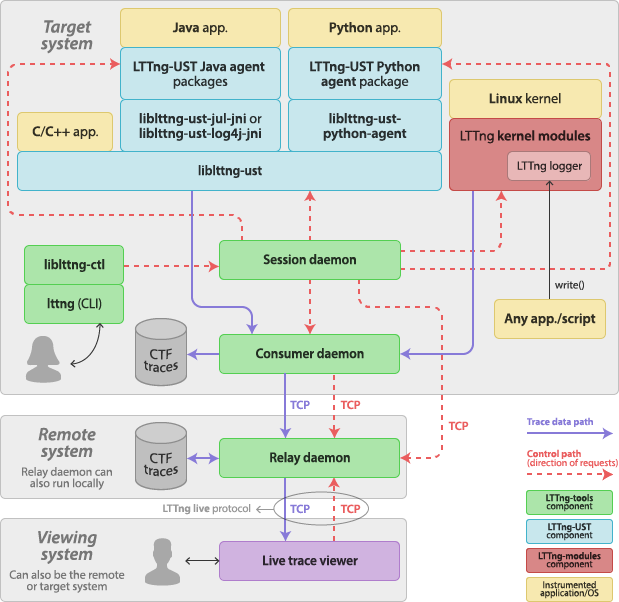
\includegraphics[height=0.8\textheight]{slides/debugging-system-wide-profiling/lttng_graph.png}\\
    \tiny Image credits: \url{https://lttng.org/}
  \end{center}
\end{frame}

\begin{frame}
  \frametitle{Tracepoints with {\em LTTng} }
  \begin{itemize}
    \item LTTng can use and trace the following instrumentation points:
    \begin{itemize}
      \item LTTng kernel tracepoints
      \item kprobes and kretprobes
      \item Linux kernel system calls
      \item Linux user space probe
      \item User space LTTng tracepoints
    \end{itemize}
    \item LTTng works with a session daemon that receive all events from kernel
          and userspace LTTng tracing components.
    \item Session daemon should be started as daemon and the user should be in
          the {\em tracing} group.
  \end{itemize}
\end{frame}

\begin{frame}
  \frametitle{Creating userspace tracepoints with {\em LTTng}}
  \begin{itemize}
    \item New userspace tracepoints can be defined using LTTng.
    \item Tracepoints have multiple characteristics:
    \begin{itemize}
      \item A provider namespace
      \item A name identifying the tracepoint
      \item Parameters of various types (int, char *, etc)
      \item Fields describing how to display the tracepoint parameters
            (decimal, hexadecimal, etc)
    \end{itemize}
    \item Tracepoints are defined using a tracepoint provider header file
          template and a tracepoint provider package file.
    \begin{itemize}
      \item The tracepoint provider header file template contains the definition
            of the tracepoints.
      \item The tracepoint provider package is the instantiation of the
            tracepoints.
    \end{itemize}
    \item See \href{https://lttng.org/man/3/lttng-ust/v2.13/}{LTTng-ust} manpage
          for types
  \end{itemize}
\end{frame}

\begin{frame}[fragile]
  \frametitle{Defining a {\em LTTng} tracepoint (1/2)}

  \begin{itemize}
    \item Tracepoint provider header file (\code{hello_world-tp.h}):
  \end{itemize}
  \begin{block}{}
    \begin{minted}[fontsize=\tiny]{C}
#undef LTTNG_UST_TRACEPOINT_PROVIDER
#define LTTNG_UST_TRACEPOINT_PROVIDER hello_world

#undef LTTNG_UST_TRACEPOINT_INCLUDE
#define LTTNG_UST_TRACEPOINT_INCLUDE "./hello-tp.h"

#if !defined(_HELLO_TP_H) || defined(LTTNG_UST_TRACEPOINT_HEADER_MULTI_READ)
#define _HELLO_TP_H

#include <lttng/tracepoint.h>

LTTNG_UST_TRACEPOINT_EVENT(
    hello_world,
    my_first_tracepoint,
    LTTNG_UST_TP_ARGS(
        int, my_integer_arg,
        char *, my_string_arg
    ),
    LTTNG_UST_TP_FIELDS(
        lttng_ust_field_integer(int, my_integer_field, my_integer_arg)
        lttng_ust_field_string(my_string_field, my_string_arg)
    )
)
#endif /* _HELLO_TP_H */

#include <lttng/tracepoint-event.h>
   \end{minted}
  \end{block}
\end{frame}

\begin{frame}[fragile]
  \frametitle{Defining a {\em LTTng} tracepoint (2/2)}
  \begin{itemize}
    \item Tracepoint provider package (\code{hello_world-tp.c}):
  \end{itemize}
  \begin{block}{}
    \begin{minted}[fontsize=\tiny]{C}
#define LTTNG_UST_TRACEPOINT_CREATE_PROBES
#define LTTNG_UST_TRACEPOINT_DEFINE

#include "hello-tp.h"
   \end{minted}
  \end{block}

  \begin{itemize}
    \item Tracepoint usage (\code{hello_world.c}):
  \end{itemize}
  \begin{block}{}
    \begin{minted}[fontsize=\tiny]{C}
#include <stdio.h>
#include "hello-tp.h"

int main(int argc, char *argv[])
{
    lttng_ust_tracepoint(hello_world, my_first_tracepoint, 23, "hi there!");
    return 0;
}
   \end{minted}
  \end{block}
  \begin{itemize}
    \item Compilation:
  \end{itemize}
  \begin{block}{}
    \begin{minted}[fontsize=\tiny]{console}
$ gcc hello_world.c hello_world-tp.c -llttng-ust -o hello_world
   \end{minted}
  \end{block}
\end{frame}

\begin{frame}[fragile]
  \frametitle{Generating tracepoints using \code{lttng-gen-tp}}
  \begin{itemize}
    \item Writing both the \code{.h} and \code{.c} boilerplate can be avoided
          using \code{lttng-gen-tp}.
    \item \code{lttng-gen-tp} takes a template file (\code{.tp}) as input and will
          generate both the provider header and package files (\code{.h},
          \code{.c} and \code{.o} files):
  \end{itemize}
  \begin{block}{}
    \begin{minted}[fontsize=\tiny]{C}
  LTTNG_UST_TRACEPOINT_EVENT(
    // Tracepoint provider name
    hello_world,

    // Tracepoint/event name
    first_tp,

    // Tracepoint arguments (input)
    LTTNG_UST_TP_ARGS(
        char *, text
    ),

    // Tracepoint/event fields (output)
    LTTNG_UST_TP_FIELDS(
        lttng_ust_field_string(message, text)
    )
)
   \end{minted}
  \end{block}
\end{frame}

\begin{frame}[fragile]
  \frametitle{Using {\em LTTng}}
  \begin{block}{}
    \begin{minted}[fontsize=\small]{console}
$ lttng create my-tracing-session --output=./my_traces
$ lttng list --kernel
$ lttng list --userspace
$ lttng enable-event --userspace hello_world:my_first_tracepoint
$ lttng enable-event --kernel --syscall open,close,write
$ lttng start
$ /* Run your application or do something */
$ lttng destroy
$ babeltrace2 ./my_traces
   \end{minted}
  \end{block}
\end{frame}

\begin{frame}[fragile]
  \frametitle{Remote tracing with {\em LTTng}}
  \begin{itemize}
    \item LTTng allows to record traces over the network.
    \item Useful for embedded systems with limited storage capabilities.
    \item On the remote computer, run \code{lttng-relayd} command
  \end{itemize}
  \begin{block}{}
    \begin{minted}[fontsize=\small]{console}
$ lttng-relayd --output=${PWD}/traces
   \end{minted}
  \end{block}
  \begin{itemize}
    \item Then on the target, at session creation, use the \code{--set-url}
  \end{itemize}
  \begin{block}{}
    \begin{minted}[fontsize=\small]{console}
$ lttng create my-session --set-url=net://remote-system
   \end{minted}
  \end{block}
  \begin{itemize}
    \item Traces will then be recorded directly on the remote computer.
  \end{itemize}
\end{frame}

\begin{frame}[fragile]
  \frametitle{Choosing the right tool}
  \begin{itemize}
    \item Before starting to profile or trace, one should know which type of
          tool to use.
    \item This choice is guided by the level of profiling
    \item Often start by analyzing/optimizing the application level using
          application tracing/profiling tools (valgrind, perf, etc).
    \item Then analyze user space + kernel performance
    \item Finally, trace or profile the whole system if the performance problems
          happens only when running under a loaded system.
    \begin{itemize}
      \item For "constant" load problems, snapshot tools works fine.
      \item For sporadic problems, record traces and analyze them.
    \end{itemize}
  \end{itemize}
\end{frame}

\setuplabframe
{System wide profiling}
{
  Profiling a system from userspace to kernel space
  \begin{itemize}
    \item Profiling with ftrace, uprobes and kernelshark
    \item Profiling with LTTng and trace-compass
    \item Profiling with perf
  \end{itemize}
}
